\chapter{Evaluation}
\label{chapter:evaluation}

\section{Setup}

We want to measure cold start latency and action execution time across all our evaluations. To that end, we utilize OpenWhisk's activation record, which is a collection of data resulting from each action invocation.  Recall that OpenWhisk either initializes and runs the action, in the case of a cold start, or skips the initilization and runs it in a warm container. In the cold start case, OpenWhisk additionally attaches an \inl{initTime} annotation to the record, which is the cold start latency. The record also contains a \inl{duration} field which is the duration of the entire execution, including a potential cold start time. In figure \ref{fig:evaluation-time-measurement} we show an overview of the two measurements we calculate.

\begin{figure}
    \begin{center}
        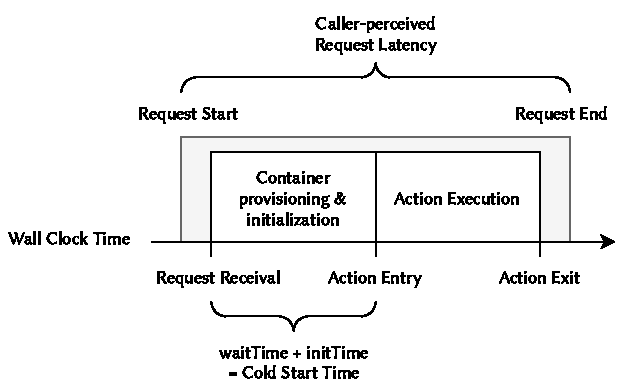
\includegraphics{figures/EvaluationTimeMeasurement.pdf}
    \end{center}
    \caption{The two durations we calculate to measure the system's performance.}
    \label{fig:evaluation-time-measurement}
\end{figure}

% With this setup alone, it is difficult to measure the cold start latency, since end - start would include the execution time. To lift this restriction, we additionally measure the wall clock time inside the action, when it enters its main function. Furthermore -- to maximize precision -- we also measure the timestamp at which the main function exits and ignore the activation end timestamp as a result. That leads us to our setup in figure \ref{fig:evaluation-time-measurement}. Now we can accurately measure the time it takes to get the underlying container technology initialized by taking the difference of the entry and start timestamp.

% start - end includes Wasm module's memory allocation and serialization, could mention that and reference its description in the design chapter

% Possibly cite https://www.sciencedirect.com/science/article/pii/B9780124201583000137?via%3Dihub

The lack of existing research on serverless workloads -- particularly whether they're CPU- or I/O-bound -- indicates that we need to examine the system for both types.

There are many papers measuring performance of serverless systems.

\begin{itemize}
    \item \citeauthor{McGrath2017} use concurrency and backoff tests. The concurrency test starts by issuing a request to the platform and reissues it as soon as it completes. At a fixed interval, it adds another request up to an upper bound. The performance metric is responses per second. The backoff test measures cold start times by issuing single requests at increasing intervals, in order to trigger the platforms deallocation of warm containers \cite{McGrath2017}.
    \item \citeauthor{Hall2019} characterize serverless function access patterns based on a real-world scenario. They describe three different patterns: Non-concurrent requests from a single client; multiple clients making a single request, possibly concurrent; multiple clients making multiple concurrent requests \cite{Hall2019}.
\end{itemize}

In the interest of reducing complexity, we will run multiple evaluations and measure for the least amount of dimensions. Those evaluations are:

\begin{enumerate}
    \item To evaluate the cold start latency we will send single requests to our deployment on an edge device with varying modules, representing either CPU- or I/O-bound actions. We repeat this measurement for all our Wasm runtimes. We use a similar approach as \citeauthor{McGrath2017} in their backoff test. In our case, we can fix the interval, since we can configure the deallocation time as well. This measurement will aid in answering research question 1.
    \item To evaluate the performance of the system we will run concurrent requests against an edge device under a mixed workload consisting of equal amounts of CPU- and I/O-bound actions. We repeat this measurement for all our Wasm runtimes. We use the approach by \citeauthor{McGrath2017} in their concurrency test, and pick workload types at random. This is to ensure that we evaluate the system for both types and because it is closer to a real-world scenario than measuring one type in isolation. It is also similar to the approach of \citeauthor{Hall2019}, in that we also have multiple concurrent requests but multiple clients are replaced by diverse workload types, which is likely equivalent. This measurement will help us answer research question 2.
    \item Since serverless systems keep their containers warm for some time, the memory they claim is of interest. We will measure the memory footprint of keeping containers warm. \todo{Memory footprint of container during execution? Is that interesting?} We measure this footprint only on the container technology. For Docker we use \inl{docker stats} and for our executor we use \inl{heaptrack} \footnote{\url{https://github.com/KDE/heaptrack}}. This measurement allows answering research question 3.
\end{enumerate}

Finally, all measurements will lead us to a conclusion on research question 4.
